\documentclass[a4paper,11pt]{scrartcl}

\usepackage{style}

\titlehead{Graduate Seminar on Advanced Algebra \hfill Jendrik Stelzner \hfill December 12, 2019}
\title{Jordan Quiver, Part~I}
\subtitle{Talk~10 on Hall~Algebras and Quantum Groups}
\author{}
\date{}

\begin{document}

\maketitle

\vspace{-4em}





\section{The Jordan Quiver and its Nilpotent Representations}

\begin{definition}
  The \defemph{Jordan quiver} is the quiver that consists of a single vertex and a single edge, which is necessarily a loop.
\end{definition}

Throughout this talk the Jordan quiver is denoted by~$Q$.
%Its single vertex is denoted by~$1$, and its single edge by~$\alpha$.
See \cref{jordan quiver} for a visualization.
\begin{figure}[tb]
  \centering
  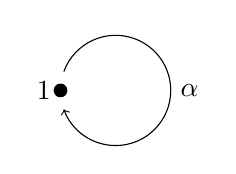
\begin{tikzpicture}
    \draw[fill = black] (-0.7 ,0) circle (0.08) node[anchor = east] {$1$};
    \draw ([shift=(160 : 0.7)]0, 0) arc (160 : 0: 0.7) node [anchor = west] {$\alpha$};
    \draw[->] (0.7, 0)  arc (0 : -160 :  0.7);
    %\draw[-{libertinustip[length=5pt]}, thick] (-0.7, 0) arc (160 :  20   : 0.7);
    %\draw[thick] ( 0.7, 0) arc (0   : -180 : 0.7);
  \end{tikzpicture}
  \caption{The Jordan quiver~$Q$.}
  \label{jordan quiver}
\end{figure}
In the following we write~$\kf$ to mean a field or~$\Finite_1$.

A representation of the Jordan~quiver over~$\kf$ is the same as a pair~$(V,f)$ consisting of a~\vectorspace{$\kf$}~$V$ together with an endomorphism~$f$ of~$V$.
A homomorphism of representations~$\varphi \colon (V,f) \to (W,g)$ is then precisely a homomorphism of vector spaces~$\varphi \colon V \to W$ that makes the following square diagram commute:
\[
  \begin{tikzcd}[column sep = large]
    V
    \arrow{r}[above]{\varphi}
    \arrow{d}[left]{f}
    &
    W
    \arrow{d}[right]{g}
    \\
    V
    \arrow{r}[below]{\varphi}
    &
    W
  \end{tikzcd}
\]
If~$(V, f) \cong (W, g)$ then in particular~$V \cong W$ as vector spaces.
So to understand the isomorphism classes of~\representations{$Q$} over~$\kf$ we may assume that~$V = W$.
The commutativity of the above square diagram, together with the requirement that~$\varphi$ is an isomorphism, means precisely that the endomorphisms~$f$,~$g$ of~$V$ are similar.
We hence find that that the isomorphism classes of~\representations{$Q$} over~$\kf$ correspond one-to-one to conjugacy classes of endomorphisms of~\vectorspaces{$\kf$}.

Suppose that~$V$ is finite-dimensional.
If~$\kf$ is a field then these conjugacy classes are can be understood via the rational canonical form.
In the case that~$\kf$ is also algebraically closed, or that it is~$\Finite_1$, or that we are interested only in nilpotent endomorphisms, one can use the usual Jordan normal form.

\begin{recall}
  A representation~$V = ((V_i)_{i \in \Gamma_0}, (f_\alpha)_{\alpha \in \Gamma_1})$ of a quiver~$\Gamma = (\Gamma_0, \Gamma_1)$ is \defemph{nilpotent} if there exists some~$N \geq 0$ such that for every path~$\alpha_n, \dotsc, \alpha_1$ in~$\Gamma$ of length~$n \geq N$ we have~$f_{\alpha_n} \circ \dotsb \circ f_{\alpha_1} = 0$.
  (See \cite[Definition~4.4]{quiver_reps_F1}.)

  If~$\Gamma$ is finite and has no oriented cycles then every representation of~$\Gamma$ is nilpotent.
\end{recall}

A representation~$(V, f)$ of the Jordan quiver is nilpotent if and only if the endomorphism~$f$ is nilpotent.
We will in the rest of this talk restrict our attention to finite-dimensional, nilpotent representations of the Jordan quiver.

\begin{definition}
  The category~$\Repnil(Q, \kf)$ is the full subcategory of~$\Rep(Q, \kf)$ whose objects are the finite-dimensional, nilpotent representations of~$Q$ over~$\kf$.
  The set of isomorphism classes in~$\Repnil(Q, \kf)$ is denoted by~$\Iso(Q, \kf)$.
\end{definition}

Every nilpotent endomorphism on a finite-dimensional~\vectorspace{$\kf$} admits a Jordan normal form.
We can therefore classify the isomorphism classes of~$\Repnil(Q, \kf)$:
For every dimension~$d \geq 0$ let
\[
  \Nil_d
  \defined
  \left(
    \kf^d,
    \begin{bmatrix}
      0 & 1       &         &   \\
        & \ddots  & \ddots  &   \\
        &         & \ddots  & 1 \\
        &         &         & 0
    \end{bmatrix}
  \right)
\]
if~$\kf$ is a field, and let
\[
  \Nil_d
  \defined
  (
    \{ 0, 1, \dotsc, d \},
    [d \mapsto (d-1) \mapsto (d-2) \mapsto \dotsb \mapsto 1 \mapsto 0 \mapsto 0]
  )
\]
if~$\kf = \Finite_1$.
For every tupel~$(d_1, \dotsc d_n)$ of dimensions~$d_i \geq 0$ let
\[
  \Nil_{(d_1, \dotsc, d_n)}
  \defined
  \Nil_{d_1} \oplus \dotsb \oplus \Nil_{d_n} \,.
\]
See \cref{nilpotent representation example} for a visualization of~$\Nil_{(d_1, \dotsc, d_n)}$.
\begin{figure}[tb]
  \centering
    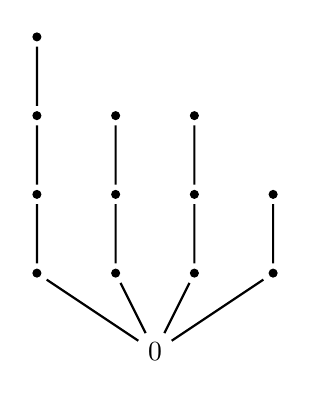
\begin{tikzpicture}
      % origin
      \node at (0,0) (Z) {$0$};
      % first line
      \node at (-1.5,1) (A1) {};
      \node at (-1.5,2) (A2) {};
      \node at (-1.5,3) (A3) {};
      \node at (-1.5,4) (A4) {};
      \draw[fill = black] (A1) circle (0.05);
      \draw[fill = black] (A2) circle (0.05);
      \draw[fill = black] (A3) circle (0.05);
      \draw[fill = black] (A4) circle (0.05);
      \draw[thick] (A4) -- (A3) -- (A2) -- (A1) -- (Z);
      % second line
      \node at (-0.5,1) (B1) {};
      \node at (-0.5,2) (B2) {};
      \node at (-0.5,3) (B3) {};
      \draw[fill = black] (B1) circle (0.05);
      \draw[fill = black] (B2) circle (0.05);
      \draw[fill = black] (B3) circle (0.05);
      \draw[thick] (B3) -- (B2) -- (B1) -- (Z);
      % third line
      \node at (0.5,1) (C1) {};
      \node at (0.5,2) (C2) {};
      \node at (0.5,3) (C3) {};
      \draw[fill = black] (C1) circle (0.05);
      \draw[fill = black] (C2) circle (0.05);
      \draw[fill = black] (C3) circle (0.05);
      \draw[thick] (C3) -- (C2) -- (C1) -- (Z);
      % fourth line
      \node at (1.5,1) (D1) {};
      \node at (1.5,2) (D2) {};
      \draw[fill = black] (D1) circle (0.05);
      \draw[fill = black] (D2) circle (0.05);
      \draw[thick] (D2) -- (D1) -- (Z);
    \end{tikzpicture}
    \qquad\qquad
    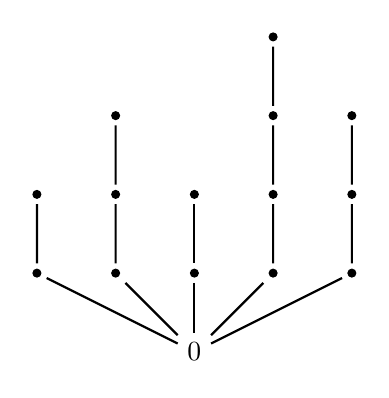
\begin{tikzpicture}
      % origin
      \node at (0,0) (Z) {$0$};
      % first line
      \node at (-2,1) (A1) {};
      \node at (-2,2) (A2) {};
      \draw[fill = black] (A1) circle (0.05);
      \draw[fill = black] (A2) circle (0.05);
      \draw[thick] (A2) -- (A1) -- (Z);
      % second line
      \node at (-1,1) (B1) {};
      \node at (-1,2) (B2) {};
      \node at (-1,3) (B3) {};
      \draw[fill = black] (B1) circle (0.05);
      \draw[fill = black] (B2) circle (0.05);
      \draw[fill = black] (B3) circle (0.05);
      \draw[thick] (B3) -- (B2) -- (B1) -- (Z);
      % third line
      \node at (-0,1) (C1) {};
      \node at (-0,2) (C2) {};
      \draw[fill = black] (C1) circle (0.05);
      \draw[fill = black] (C2) circle (0.05);
      \draw[thick] (C2) -- (C1) -- (Z);
      % fourth line
      \node at (1,1) (D1) {};
      \node at (1,2) (D2) {};
      \node at (1,3) (D3) {};
      \node at (1,4) (D4) {};
      \draw[fill = black] (D1) circle (0.05);
      \draw[fill = black] (D2) circle (0.05);
      \draw[fill = black] (D3) circle (0.05);
      \draw[fill = black] (D4) circle (0.05);
      \draw[thick] (D4) -- (D3) -- (D2) -- (D1) -- (Z);
      % fifth line
      \node at (2,1) (E1) {};
      \node at (2,2) (E2) {};
      \node at (2,3) (E3) {};
      \draw[fill = black] (E1) circle (0.05);
      \draw[fill = black] (E2) circle (0.05);
      \draw[fill = black] (E3) circle (0.05);
      \draw[thick] (E3) -- (E2) -- (E1) -- (Z);
    \end{tikzpicture}
    \caption{The representations~$\Nil_{(4,3,3,2)}$ and~$\Nil_{(2, 3, 2, 4, 3)}$ over~$\Finite_1$.}
  \label{nilpotent representation example}
\end{figure}

\begin{proposition}[Jordan normal form for nilpotent endomorphisms]
  \label{jordan normal form applied to reps}
  Let~$\kf$ be any field.
  \begin{enumerate}
    \item
      Every finite-dimensional, nilpotent representation of~$Q$ over~$\kf$ is isomorphic to a representation of the form~$\Nil_{(d_1, \dotsc, d_n)}$ for some~$n \geq 0$ and~$d_1, \dotsc, d_n \geq 1$.
    \item
      Two such representations~$\Nil_{(d_1, \dotsc, d_n)}$ and~$\Nil_{(d'_1, \dotsc, d'_m)}$ are isomorphic if and only if~$n = m$ and the tuples~$(d_1, \dotsc, d_n)$ and~$(d'_1, \dotsc, d'_m)$ are the same up to permutation.
  \end{enumerate}
\end{proposition}

We can reformulate the above \lcnamecref{jordan normal form applied to reps} in terms of partitions:

\begin{definition}
  For every~$n \geq 0$ let~$\Par(n)$ be the set of partition of the number~$n$, i.e.\
  \[
    \Par(n)
    \defined
    \{
      (\lambda_1, \dotsc, \lambda_l)
    \suchthat
      \lambda_1 \geq \dotsb \geq \lambda_l \geq 1,
      \lambda_1 + \dotsb + \lambda_l = n
    \} \,.%
    \footnote{
      We want to point out that in this talk we do not allow a partition to contain zero as an entry.
      This is done purely for technical reasons.
    }
  \]
  The set of all partitions is denoted by
  \[
    \Par
    \defined
    \coprod_{n \geq 0} \Par(n) \,.
  \]
\end{definition}


\begin{corollary}
  \label{representatives via partitions}
  The representations~$\Nil_\lambda$ with~$\lambda \in \Par$ form a set of representatives for~$\Iso(Q, \kf)$.
\end{corollary}

We find in particular that the category~$\Repnil(Q, \kf)$ admits only finitely many isomorphism classes of objects.




\section{The Hall~Algebra of the Jordan Quiver over~$\Finite_q$}

We consider for~$\kf$ the finite field~$\Finite_q$.

\begin{proposition}
  The category~$\Repnil(Q)$ is hereditary.
\end{proposition}

\begin{proof}
  ?????
\end{proof}

\begin{lemma}
  Let~$S \defined \Nil_1$.
  \begin{enumerate}
    \item
      The representation~$S$ is the unique simple object of~$\Repnil(Q, \Finite_q)$ (up to isomorphism).
    \item
      The Groethendieck group~$\GrGr_0(\Repnil(Q, \Finite_q))$ is freely generated by the class~$\class{S}$.
      Thus
      \[
        \GrGr_0(\Repnil(Q, \Finite_q))
        \cong
        \Integer
      \]
      via the map~$\class{M} \mapsto \dim(M)$.
    \item
      We have both~$\Hom(S, S) = \Finite_q$ and~$\Ext^1(S,S) = \Finite_q$.
  \end{enumerate}
\end{lemma}

\begin{proof}
  \leavevmode
  \begin{enumerate}
    \item
      The indecomposable objects of~$\Repnil(Q, \Finite_q)$ are precisely~$\Nil_i$ with~$i \geq 1$.
      The representation~$\Nil_i$ has (up to isomorphism) the subrepresentations~$\Nil_j$ with~$j = 0, \dotsc, i$.
      Thus only~$\Nil_1$ is simple.
    \item
      This follows from the previous assertion since~ each objects of~$\Repnil(Q, \Finite_q)$ admits a composition series, whose composition factors are necessarily~$S$.
    \item
      We have~$\Hom(S, S) = \Finite_q$ because~$S$ is one-dimensional.
      
      Computation of~$\Ext^1(S,S)$:
      Can be done via homological algebra or by explicit counting of Yoneda extensions.
      (It still needs to be decided which one to use.)
    \qedhere
  \end{enumerate}
\end{proof}

\begin{corollary}
  The Euler form of~$\Repnil(Q, \Finite_q)$ is trivial.
\end{corollary}

\begin{proof}
  Let~$K \defined \GrGr_0(\Repnil(Q, \Finite_q))$.
  We can regard the Euler form of~$\Repnil(Q, \Finite_q)$ as a bilinear form
  \[
    \euler{-}{-}
    \colon
    K \times K
    \to
    \Rational^\times \,.
  \]
  Since~$S$ is a generator of~$K$ is sufficies to show that~$\euler{S}{S} = 1$.
  This holds true because
  \[
    \euler{S}{S}
    =
    \Bigl( \counting {\Hom(S,S)} \Bigr)
    \cdot
    \Bigl( \counting \Ext^1(S,S) \Bigr)^{-1}
    =
    q \cdot q^{-1}
    =
    1 \,.
  \]
  This proves the assertion.
\end{proof}

We find from the above that~$\Repnil(Q, \Finite)$ is a abelian, finitary, hereditary category, which admits only finitely many isomorphism classes of objects (i.e.\ it is essentially finite).
We are thus well-prepared to consider the Hall algebra~$\Hall(Q, \Finite_q)$.
\begin{enumerate}
  \item
    The underlying vector space of~$\Hall(Q, \Finite_q)$ is free on the set of isomorphism classes,~$\Iso(Q, \Finite_q)$.
    This basis is indexed by the set of partitions~$\Par$.
  \item
    The multiplication on~$\Hall(Q, \Finite_q)$ is given by
    \[
      \class{M} \cdot \class{N}
      =
      \sum_{\class{R} \in \Iso(Q, \Finite_q)}
      C^R_{M,N} \class{R}
    \]
    where
    \[
      C^R_{M,N}
      =
      \text{number of subrepresentations~$L$ of~$R$ with~$L \cong N$ and~$R/L \cong M$} \,.
    \]
    The multiplicative neutral element of~$\Hall(Q, \Finite_q)$ is given by~$1_{\Hall(Q, \Finite_q)} = \class{0}$.
  \item
    Since the Euler form of~$\Repnil(Q, \Finite_q)$ vanishes and~$\Iso(Q, \Finite_q)$ is finite we find that Green’s product makes the Hall algebra~$\Hall(Q, \Finite_q)$ into a bialgebra.
    Its comultiplication is given by
    \[
      \Delta(\class{M})
      =
      \sum_{\class{M}, \class{N} \in \Iso(Q, \Finite_q)}
      \frac{1}{a_R} P^R_{M,N} \class{M} \tensor \class{N}
    \]
    where~$a_R$ is the size of the automorphism group~$\Aut(R)$, and~$P^R_{M,N}$ is the number of short exact sequences~$0 \to N \to R \to M \to 0$.
    % TODO: Right formula for comultiplication?
    The counit~$\varepsilon \colon \Hall(Q, \Finite_q) \to \Complex$ is given by
    \[
      \varepsilon(\class{M})
      =
      \begin{cases*}
          1
          &
          if~$M = 0$,
          \\
          0
          &
          otherwise.
      \end{cases*}
    \]
  \item
    We have a grading on~$\Hall(Q, \Finite_q)$ over the Grothendieck group~$\GrGr(\Repnil(Q, \Finite_q)) \cong \Integer$, given by
    \[
      \deg( \class{M} )
      =
      \dim(M) \,.
    \]
    This grading makes~$\Hall(Q, \Finite_q)$ into a graded bialgebra.
  \item
    The graded bialgebra~$\Hall(Q, \Finite_q)$ is connected (i.e.\ its degree zero part is the ground field).
    It is therefore already a graded Hopf algebra.
\end{enumerate}

We will in the rest of this talk be mostly concerned with the upcoming Hall~algebra~~$\Hall(Q, \Finite_1)$.
But we will here compute at least some of the structure constants of~$\Hall(Q, \Finite_q)$.
For this we follow \cite[Example~2.2]{schiffmann_hall}.


\begin{recall}
  For~$k \in \Natural$ the \defemph{quantum integer}~$\qnum{k}_q$ is given by
  \[
    \qnum{k}_q
    =
    1 + q + q^2 + \dotsb + q^{k-1}
    =
    \frac{q^k - 1}{q - 1} \,.
  \]
  We have~$\qnum{0}_q = 0$ and~$\qnum{1}_q = 1$.
  The \defemph{quantum factorial} is given by
  \[
    \qnum{k}_q !
    =
    \qnum{k}_q \qnum{k-1}_q \dotsm \qnum{1}_q \,.
  \]
  For~$k, l \in \Natural$ the \defemph{quantum binomial} is given by
  \[
    \qbinomial{k}{l}_q
    =
    \frac{\qnum{k}_q \dotsm \qnum{k-l+1}_q}{\qnum{l}_q!} \,.
  \]
  If~$l > k$ then this is zero, and if~$l \leq k$ then the quantum binomial can also be expressed as
  \[
    \qbinomial{k}{l}_q
    =
    \frac{\qnum{k}_q!}{\qnum{l}_q! \, \qnum{k-l}_q!} \,.
  \]
  The quantum binomial satsfies the recursive relation
  \[
    \qbinomial{k}{l}_q
    =
    q^l \qbinomial{k-1}{l}_q
    +
    \qbinomial{k-1}{l-1}_q
  \]
  for all~$k, l \in \Natural$.
  It hence follows by induction that the quantum binomial~$\qbinomial{k}{l}_q$ is a polynomial in~$q$ with natural coefficients, i.e.
  \[
    \qbinomial{k}{l}_q
    \in
    \Natural[q] \,.
  \]
  By taking the limit~$q \to 1$ (i.e.\ by setting~$q$ equal to~$1$) the quantum integer~$\qnum{k}$ becomes the usual integer~$k$, the quantum factorial~$\qnum{k}_q!$ becomes the usual factorial~$k!$ and the quantum binomial coefficient~$\qbinomial{k}{l}_q$ becomes the usual binomial~$\binom{k}{l}$.
\end{recall}

\begin{lemma}
  For all dimensions~$n, d \geq 0$ we have
  \[
    \counting {\Gr(d, n, \Finite_q)}
    =
    \qbinomial{n}{d}_q \,.
  \]
\end{lemma}

\begin{proof}
  If~$d > n$ then both numbers are zero, so suppose that~$d \leq n$.  
  Let
  \[
    F_d(n)
    \defined
    (q^n - 1) \dotsm (q^n - q^{d-1})
    =
    (q-1)^d \, q^{d(d-1)/2} \, \qnum{n}_q \dotsm \qnum{n-d+1}_q
  \]
  This is the number of linear independent tupels~$(v_1, \dotsc, v_d)$ of vectors in~$\Finite_q^n$.
  We find that
  \[
    \counting {\Gr(d, n, \Finite_q)}
    =
    \frac{ F_d(n) }{ \counting {\GL(d, \Finite_q)} } \,.
  \]
  We have~$\counting {\GL(d, \Finite_q)} = F_d(d)$ and thus
  \[
    \counting {\Gr(d, n, \Finite_q)}
    =
    \frac{ F_d(n) }{ F_d(d) }
    =
    \frac{ \qnum{n}_q \dotsm \qnum{n-d+1}_q }{ \qnum{d}_q \dotsm  \qnum{1}_q }
    =
    \frac{ \qnum{n}_q \dotsm \qnum{n-d+1}_q }{ \qnum{d}_q! }
    =
    \qbinomial{n}{d}_q \,,
  \]
  as claimed.
\end{proof}

\begin{example}
  For any three partition~$\lambda, \mu, \kappa \in \Par$ we abbreviate the structure constant
  \[
    C^{\Nil_{\kappa}}_{\Nil_{\lambda}, \Nil_{\mu}}
  \]
  as~$C^{\kappa}_{\lambda,\mu}$.
  \begin{enumerate}
    \item
      Let~$\lambda = (1^n)$ and~$\mu = (1^m)$.
      We consider the partition~$\kappa \defined (1^{n+m})$.
      The action of the edge of the Jordan quiver~$Q$ on the representations~$\Nil_\lambda$,~$\Nil_\mu$ and~$\Nil_\kappa$ is trivial.
      We thus find that every~\dimensional{$m$} linear subspace~$L$ of~$\Nil_{\kappa}$ satisfies the conditions~$L \cong \Nil_\mu$ and~$\Nil_\kappa / L \cong \Nil_\lambda$.
      The structure constant~$C^{\kappa}_{\lambda, \mu}$ is therefore given by
      \begin{align*}
        C^{\kappa}_{\lambda, \mu}
        &=
        \text{number of~\dimensional{$m$} linear subspaces of~$\Nil_{\kappa}$}
        \\
        &=
        \text{number of~\dimensional{$m$} linear subspaces of~$\Finite_q^{n+m}$}
        \\
        &=
        \counting {\Gr(m, n+m, \Finite_q)}
        \\
        &=
        \qbinomial{n+m}{m}_q \,.
      \end{align*}

      We see in particular that~$C^{\kappa}_{\lambda, \mu}$ depends is a polynomial way on~$q$. 
      We have for example
      \[
        C^{(1^{n+1})}_{(1^n),(1)}
        =
        \counting {\Gr(1, n+1, \Finite_q)}
        = 
        \counting {\Proj^n(\Finite_q)}
        =
        \frac{ q^{n+1} - 1 }{ q - 1 }
        =
        [n+1]_q
        =
        1 + q + \dotsb + q^n \,,
      \]
      and also
      \begin{align*}
        C^{(1^{n+2})}_{(1^n),(1,1)}
        &=
        \qbinomial{n+2}{2}_q
        =
        \frac{[n+2]_q [n+1]_q}{[2]_q}
        \\
        &=
        \frac{ (1 + q + \dotsb + q^n) (1 + q + \dotsb + q^{n+1}) }{ 1 + q }
        \\
        &=
        \begin{cases*}
          (1 + q + \dotsb + q^n) (1 + q^2 + \dotsb + q^n)
          &
          if~$n$ is even,
          \\
          (1 + q^2 + \dotsb + q^{n-1}) (1 + q + \dotsb + q^{n+1})
          &
          if~$n$ is odd.
        \end{cases*}
%        \\
%        &=
%        \begin{cases*}
%          \begin{aligned}
%            1 + q
%            &+ 2 (q^2 + q^3)
%            + \dotsb
%            + \biggl( 1+\frac{n}{2} \biggr) q^n
%            \\
%            &+ \dotsb
%            + 2 ( q^{2n-3} + q^{2n-2} )
%            + q^{2n-1} + q^{2n}
%          \end{aligned}
%          &
%          if~$n$ is even,
%          \\[0.5em]
%          \begin{aligned}
%            1 + q
%            &+ 2 ( q^2 + q^3 )
%            + \dotsb
%            + \biggl( 1+\frac{n+1}{2} \biggr) (q^{n-1} + q^n + q^{n+1})
%            \\
%            &+ \dotsb
%            + 2 ( q^{2n-3} + q^{2n-2} )
%            + q^{2n-1} + q^{2n}
%          \end{aligned}
%          &
%          if~$n$ is odd.
%        \end{cases*}
      \end{align*}
    \item
      Let now~$\lambda = (n)$ and~$\mu = (m)$.
      We consider the partition~$\kappa = (n+m)$. 
      The representation$~\Nil_{\kappa}$ has the standard basis~$e_1, \dotsc, e_{n+m}$, and the subrepresentations of~$\Nil_{\kappa}$ are given by~$\gen{e_1, \dotsc, e_i}$ for~$i = 0, \dotsc, n+m$.
      The subrepresentations~$L \defined \gen{e_1, \dotsc, e_m}$ is the unique one that is isomorphic to~$\Nil_\mu$, and its quotient~$\Nil_\kappa / L$ is isomorphic to~$\Nil_\lambda$.
      Thus
      \[
        C^{(n+m)}_{(n),(m)}
        =
        1 \,.
      \]
    \item
      Let us compute the coefficients~$C^{(2,1)}_{(1),(2)}$ and~$C^{(2,1)}_{(2),(1)}$.
      We use for~$\Nil_{(2,1)}$ the basis~$e_1, e_2, e_3$ with~$\alpha e_1 = e_2$ and~$\alpha e_2 = \alpha e_3 = 0$ where~$\alpha$ denotes the loop of~$Q$.
      See \cref{basis for 2 1}.
      \begin{figure}[tb]
        \centering
          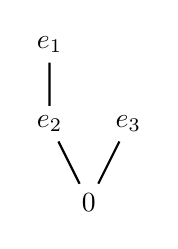
\begin{tikzpicture}
            % origin
            \node at (0,0) (Z) {$0$};
            % first line
            \node at (-0.5,2) (A1) {$e_1$};
            \node at (-0.5,1) (A2) {$e_2$};
            \draw[thick] (A1) -- (A2) -- (Z);
            % second line
            \node at (0.5,1) (B1) {$e_3$};
            \draw[thick] (B1) -- (Z);
          \end{tikzpicture}
          \caption{The representations~$\Nil_{(2,1)}$ over~$\Finite_q$.}
        \label{basis for 2 1}
      \end{figure}

      The coefficient~$C^{(2,1)}_{(1),(2)}$ is the number of subrepresentations~$L$ of~$\Nil_{(2,1)}$ with~$L \cong \Nil_2$ and~$\Nil_{(2,1)}/L \cong \Nil_1$.
      The condition~$L \cong \Nil_2$ means that~$L$ is cyclically generated by a vector~$v = a e_1 + b e_2 + c e_3$ with~$a \neq 0$.
      We may assume that~$a = 1$.
      Then
      \[
        \gen{v}_{\Finite_q Q}
        =
        \gen{ v , \alpha v }_{\Finite_q}
        =
        \gen{ e_1 + b e_2 + c e_3, e_2 }_{\Finite_q}
        =
        \gen{ e_1 + c e_3, e_2 } \,.
      \]
      For any such subrepresentation~$L$ the quotient~$\Nil_{(2,1)}/L$ is one-dimensional and thus isomorphic to~$\Nil_1$.
      We get for every coefficient~$c \in \Finite_q$ a different representation.
      Hence
      \[
        C^{(2,1)}_{(1),(2)}
        =
        \counting \Finite_q
        =
        q \,.
      \]

      The coefficient~$C^{(2,1)}_{(1),(2)}$ is the number of subrepresentations~$L$ of~$\Nil_{(2,1)}$ with~$L \cong \Nil_1$ and~$\Nil_{(2,1)}/L \cong \Nil_2$.
      The condition~$L \cong \Nil_1$ means that~$L$ is cyclically generated by a nonzero vector~$v = b e_2 + c e_3$ with~$a \neq 0$.

      If~$b \neq 0$ then we may assume that~$b = 1$, so that~$v = e_2 + c e_3$.
      Then~$\Nil_{(2,1)}/L$ has the basis vectors~$\class{e_1}$,~$\class{e_3}$ with~$\alpha \class{e_1} = - c \class{e_3}$ and~$\alpha \class{e_3} = 0$.
      Thus~$\Nil_{(2,1)}/L \cong \Nil_2$ if~$c \neq 0$ and~$\Nil_{(2,1)}/L \cong \Nil_{(1,1)}$ if~$c = 0$.
      In the case~$b \neq 0$ we thus have~$q - 1$ choices for~$L$.

      If~$b = 0$ then~$c \neq 0$ and we may assume that~$c = 1$.
      Then~$v = e_3$ and thus
      Then~$\Nil_{(2,1)}/L \cong \Nil_2$.

      We thus find that there are~$q$ choices for~$L$, i.e
      \[
        C^{(2,1)}_{(2),(1)}
        =
        q \,.
      \]
    \item
      One finds in the same way as above that more generally
      \[
        C^{(n, 1)}_{(n), (1)}
        =
        q
        =
        C^{(n, 1)}_{(1), (n)}
      \]
      for every~$n \geq 2$.
  \end{enumerate}
  We observe that in the above examples we always have~$C^{\kappa}_{\lambda, \mu} = C^{\kappa}_{\mu, \lambda}$.
  We will see in next week’s talk that the Hall algebra~$\Hall(Q, \Finite_q)$ is indeed commutative, which means precisely that~$C^\kappa_{\lambda, \mu} = C^\kappa_{\mu, \lambda}$ for any three partitions~$\lambda, \mu, \kappa \in \Par$.
\end{example}





\section{The Hall~Algebra of the Jordan Quiver over~$\Finite_1$}

We will now consider the case that~$\kf$ is~$\Finite_1$.
We have seen in last week’s talk how to construct the Hall algebra of~$Q$ over~$\Finite_1$:

\begin{recall}
  The Hall~algebra~$\Hall(Q, \Finite_1)$ is a graded, cocommutative Hopf algebra (over the ground field~$\Complex$).
  Its structure is given as follows:
  \begin{itemize}
    \item
      The underlying vector space of~$\Hall(Q, \Finite_1)$ is the free~\vectorspace{$\Complex$} on the set~$\Iso(Q, \Finite_1)$.
      The set~$\Iso(Q, \Finite_1)$ is indexed by the set of partitions~$\Par$.
    \item
      The grading of~$\Hall(Q, \Finite_1)$ is given by~$\Hall(Q, \Finite_1)_d = \gen{ \class{M} \suchthat \dim(M) = d }_{\Complex}$.
    \item
      The multiplication of$~\Hall(Q, \Finite_1)$ is given by
      \[
        \class{M} \cdot \class{N}
        \defined
        \sum_{\class{R} \in \Iso(Q, \Finite_1)}
        C^R_{M,N} \class{R}
      \]
      where the structure coefficients~$C^R_{M,N}$ are given by
      \[
        C^R_{M,N}
        =
        \counting
        \{
          \text{subrepresentations~$L$ of~$R$}
        \suchthat
          L \cong N, R/L \cong M
        \} \,.
      \]
    \item
      The multiplicative neutral element of~$\Hall(Q, \Finite_1)$ is given by~$1_{\Hall(Q, \Finite_1)} = \class{0}$.
    \item
      The comultiplication of~$\Hall(Q, \Finite_1)$ is given by
      \[
        \Delta( \class{M} )
        =
        \sum_{
          \substack{
            \class{R}, \class{L} \in \Iso(Q, \Finite_1) \\
            M \cong R \oplus L
          }
        }
        \class{R} \tensor \class{L} \,.
      \]
  \end{itemize}
  We see in particular that an isomorphism class~$\class{M}$ is primitive in~$\Hall(Q, \Finite_1)$ if and only if the representation~$M$ is indecomposable.
  We have seen that more generally the Lie algebra of primitive elements of~$\Hall(Q, \Finite_1)$ has a basis consisting of all such~$\class{M}$.
\end{recall}

\begin{example}
  \label{computing multiplication over F1}
  We can again compute some structure constants:
  \begin{enumerate}
    \item
      Let again~$\lambda = (1^n)$ and~$\mu = (1^m)$, and consider~$\kappa = (1^{n+m})$.
      We find as before that
      \[
        C^{\kappa}_{\lambda, \mu}
        =
        \text{number of~\dimensional{$m$} subspaces of~$\Nil_{n+m}$}
        =
        \binom{n+m}{m} \,.
      \]
      This is the same result as before by taking the limit~$q \to 1$.
    \item
      Let again~$\lambda = (n)$ and~$\mu = (m)$ and consider~$\kappa = (n+m)$.
      We find as before that
      \[
        C^{\kappa}_{\lambda, \mu} = 1 \,.
      \]
    \item
      Let us compute the product~$\class{\Nil_i} \cdot \class{\Nil_j}$.
      We observe that if~$\class{R} \in \Iso(Q, \Finite_1)$ and~$L$ is a subrepresentation of~$R$ that is isomorphic to~$\Nil_j$ then the quotient~$R/L$ results from~$R$ by contracting one of the Jordan chains by~$j$ elements.
      % TODO: Better formulation:
      If~$R/L \cong \Nil_i$ then this means that~$R$ consists of a single Jordan chain of length~$i+j$, or of two Jordan chains of length~$i$ and~$j$ respectively.
      Thus
      \[
        \class{\Nil_i} \cdot \class{\Nil_j}
        =
        a \class{ \Nil_{(i,j)} } \,.
        +
        b \class{ \Nil_{i+j} }
      \]
      We have seen above that~$b = C^{(i+j)}_{(i),(j)} = 1$.
      The coffient~$a$ is the number of entries of~$(i,j)$ that are of length~$j$.
      Thus
      \[
        a
        =
        \begin{cases*}
          1
          &
          if~$i \neq j$,
          \\
          2
          &
          if~$i = j$.
        \end{cases*}
      \]
      Thus
      \[
        \class{\Nil_i} \cdot \class{\Nil_j}
        =
        \begin{cases*}
          \class{\Nil_{(i,j)}} + \class{\Nil_{i+j}}
          &
          if~$i \neq j$,
          \\
          2 \class{\Nil_{(i,j)}} + \class{\Nil_{i+j}}
          &
          if~$i = j$.
        \end{cases*}
      \]
      We see in particular that~$\class{\Nil_i}$ and~$\class{\Nil_j}$ commute.
    \item
      We find in the same way that for all~$i_1, \dotsc, i_r \geq 1$ and~$j \geq 1$,
      \[
        \class{ \Nil_{(i_1, \dotsc, i_r)} } \cdot \class{ \Nil_j }
        =
        a \class{ \Nil_{(i_1, \dotsc, i_r, j)} }
        +
        \sum_{\lambda} b_\lambda \class{ \Nil_\lambda } \,,
      \]
      where~$\lambda$ runs through all distinct tupels of the form~$\lambda = (i_1, \dotsc, i_k + j, \dotsc, i_r)$ with~$1 \leq k \leq r$.
      The coeffiecient~$a$ is given by
      \begin{align*}
        a
        =
        \text{how often~$j$ occurs in~$(i_1, \dotsc, i_r, j)$}
      \end{align*}
      and the coefficient of~$b_\lambda$ for~$\lambda = (i_1, \dotsc, i_k + j, \dotsc, i_r)$ are given by
      \[
        b_\lambda
        =
        \text{how often~$i_k + j$ occurs in~$\lambda$} \,.
      \]
      We have for example
      \begin{align*}
        \class{ \Nil_{(5, 3, 3, 2, 1)} } \cdot \class{ \Nil_2 }
        ={}&
          2 \class{ \Nil_{(5, 3, 3, 2, 2, 1)} }
        \\
        {}&
        + \class{ \Nil_{(7, 3, 3, 2, 1)} }
        + 2 \class{ \Nil_{(5, 5, 3, 2, 1)} }
        +   \class{ \Nil_{(5, 4, 3, 3, 1)} }
        + 3 \class{ \Nil_{(5, 3, 3, 3, 2)} } \,.
      \end{align*}
      We see by induction that~$\Hall(Q, \Finite_1)$ is generated as an algebra by the~$N_i$ with~$i \geq 1$.
  \end{enumerate}
\end{example}

\begin{corollary}
  The Hall algebra~$\Hall(Q, \Finite_1)$ is commutative.
\end{corollary}

\begin{remark}
  We have seen last week that the Hall algebra~$\Hall(Q, \Finite_1)$ is the universal enveloping algebra of its Lie algebra of primitive elements, which in turn is spanned (as a vector space) by the~$\Nil_i$.
  We have thus already seen last week that~$\Hall(Q, \Finite_1)$ is generated by the~$\Nil_i$ as an algebra.
\end{remark}

We have hence shown that~$\Hall(Q, \Finite_1)$ is a commutative, cocommutative, graded Hopf algebra
We will in the following show that it is actually the ring of symmetric functions.





\section{The Ring of Symmetric Functions}



\subsection{Definition}

For every~$k \geq 0$ we denote by
\[
  \Lambda^{(k)}
  \defined
  \Complex[x_1, \dotsc, x_k]^{\symm_k}
\]
the algebra of symmetric polynomials in~$k$ variables.
We have for every~$r \geq 0$ a homomorphism of graded algebras
\[
  \Lambda^{(k+1)} \to \Lambda^{(k)} \,,
  \quad
  f(x_1, \dotsc, x_r, x_{k+1})
  \mapsto
  f(x_1, \dotsc, x_r, 0) \,.
\]

\begin{definition}
  The \defemph{ring of symmetric functions}~$\Lambda$ is the limit
  \[
    \Lambda
    \defined
    \lim_{k \geq 0}
    \Bigl( \Lambda^{(k+1)} \to \Lambda^{(k)} \Bigr)
  \]
  in the category of graded rings.
  The elements of~$\Lambda$ are \defemph{symmetric functions}.
\end{definition}

\begin{warning}
  A symmetric function is -- contrary to its name -- not a function.
\end{warning}

Let us make the above definition more explicit:
For every~$n \geq 0$ we have
\begin{align*}
  \Lambda_n
  &=
  \lim_{k \geq 0}
  \Bigl( \Lambda^{(k+1)}_n \to \Lambda^{(k)}_n \Bigr)
  \\
  &=
  \left\{
    \bigl( f_k(x_1, \dotsc, x_n) \bigr)_{k \geq 0}
    \suchthat*
    \begin{tabular}{@{}l@{}}
      $f_k(x_1, \dotsc, x_k) \in \Lambda^{(k)}_n$ for every~$k \geq 0$ such that \\
      $f_{k+1}(x_1, \dotsc, x_k, 0) = f_k(x_1, \dotsc, x_k)$ for every~$k \geq 0$
    \end{tabular}
  \right\} \,,
\end{align*}
and we have overall
\[
  \Lambda
  =
  \bigoplus_{n \geq 0} \Lambda_n
\]
as vector spaces.
The multiplication on~$\Lambda$ is given by~$(f_k)_{k \geq 0} \cdot (g_k)_{k \geq 0} = (f_k \cdot g_k)_{k \geq 0}$ for all~$(f_k)_{k \geq 0} \in \Lambda_n$ and~$(g_k)_{k \geq 0} \in \Lambda_m$.

A homogeneous symmetric function~$f$, say of degree~$n$, is thus the same as a \enquote{consistent choice} of homogeneous symmetric polynomials~$f_k \in \Lambda^{(k)}$ of degree~$n$ for every~$k \geq 0$.
We have for every number of variables~$k \geq 0$ a homomorphism of graded algebras
\[
  \Lambda \to \Lambda^{(k)} \,,
  \quad
  f \mapsto f(x_1, \dotsc, x_k)
\]
that is given by projection onto the~\howmanyth{$k$} component.
For any two symmetric functions~$f$,~$g$ we have by construction of~$\Lambda$ that
\[
  f = g
  \iff
  \text{$f(x_1, \dotsc, x_k) = g(x_1, \dotsc, x_k)$ for every~$k \geq 0$.}
\]

\begin{example}
  We have for every number of variables~$k \geq 0$ and every degree~$n \geq 0$ the \defemph{elementary symmetric polynomial}
  \[
    e^{(k)}_n(x_1, \dotsc, x_k)
    \defined
    \sum_{1 \leq i_1 < \dotsb < i_n \leq k}
    x_{i_1} \dotsm x_{i_n} \,,
  \]
  with~$e^{(k)}_n = 0$ whenever~$n > k$.
  These polynomials are homogeneous and satisfy the conditions
  \[
    e^{(k+1)}_n(x_1, \dotsc, x_k, 0)
    =
    e^{(k)}_n(x_1, \dotsc, x_k)
  \]
  for all~$k \geq 0$.
  These elementary symmetric polynomials~$e^{(k)}_n$ with~$k \geq 0$ therefore assemble into a single homogeneous symmetric function
  \[
    e_n \in \Lambda_n \,.
  \]
  This is the~\defemph{\howmanyth{$n$} elementary symmetric function}. 

  We find similarly that the \defemph{power symmetric polynomials}
  \[
    p^{(k)}_n(x_1, \dotsc, x_k)
    \defined
    x_1^n + \dotsb + x_k^n \,,
  \]
  and the \defemph{completely homogenous symmetric polynomials}
  \[
    h^{(k)}_n(x_1, \dotsc, x_k)
    \defined
    \sum_{1 \leq i_1 \leq \dotsb \leq i_n \leq k}
    x_{i_1} \dotsm x_{i_n}
    =
    \sum \text{monomials of homogeneous degree~$n$}
  \]
  result in homogeneous symmetric functions
  \[
    p_n, h_n \in \Lambda \,.
  \]
  These are the \defemph{power symmetric functions} and \defemph{completely homogeneous symmetric functions}.
\end{example}


\begin{warning}
  The ring of symmetric functions~$\Lambda$ is \emph{not} the limit of the rings of symmetric polynomials~$\Lambda^{(k)}$ in the category of (commutative) rings.
  Indeed, the symmetric polyonmials
  \[
    f_k(x_1, \dotsc, x_k)
    \defined
    x_1 + x_1 x_2 + \dotsb + x_1 \dotsm x_k
  \]
  satisfy the compatibility condition~$f_{k+1}(x_1, \dotsc, x_k, 0) = f_k(x_1, \dotsc, x_k)$ for every~$k \geq 0$.
  But there exists no symmetric function~$f \in \Lambda$ with~$f(x_1, \dotsc, x_k) = f_k(x_1, \dotsc, x_k)$ for every~$k \geq 0$.

  An arbitrary family~$(f_k)_{k \geq 0}$ of compatible symmetric polynomials~$f_k \in \Lambda^{(k)}$ defines a symmetric function if and only if the degrees~$\deg(f_k)$ are bounded, i.e.\ if there exists some degree~$d \geq 0$ with~$\deg(f_k) \leq d$ for every~$k \geq 0$.
\end{warning}



\subsection{The Fundamental Theorem on Symmetric Functions}

The \defemph{fundamental theorem of symmetric polynomials} asserts that for every number of variables~$k \geq 0$ the elementary symmetric polynomials~$e^{(k)}_1, \dotsc, e^{(k)}_k$ form an algebraically independent generating set for the algebra of symmetric polynomials~$\Lambda^{(k)}$.
It follows from this that the completely homogeneous symmetric polynomials~$h^{(k)}_1, \dotsc, h^{(k)}_k$ form an algebraically independent generating set for~$\Lambda^{(k)}$, and one can show that the same holds true for the power symmetric polynomials~$p^{(k)}_1, \dotsc, p^{(k)}_k$.%
\footnote{
  For the elementary symmetric polynomials~$e^{(k)}_i$ and homogeneous symmetric polynomials~$h^{(k)}_i$ these statements do not only hold over the ground field~$\Complex$, but over every commutative ring.
  For the power symmetric polynomials~$p^{(k)}_i$ we need to work over a field in which the numbers~$1, \dotsc, k$ are invertible.
}

For every partition~$\lambda \in \Par$ we can consider the symmetric polynomials
\[
  e^{(k)}_\lambda
  \defined
  e^{(k)}_{\lambda_1} \dotsm e^{(k)}_{\lambda_l} \,,
  \quad
  h^{(k)}_\lambda
  \defined
  h^{(k)}_{\lambda_1} \dotsm h^{(k)}_{\lambda_l} \,,
  \quad
  p^{(k)}_\lambda
  \defined
  p^{(k)}_{\lambda_1} \dotsm p^{(k)}_{\lambda_l} \,.
\]
We have just formulated that the symmetric polynomials~$e^{(k)}_\lambda$ for~$\lambda \in \Par$ with length~$\leq k$ form a vector space basis for~$\Lambda^{(k)}$, and similarly for~$h^{(k)}_\lambda$ and~$p^{(k)}_\lambda$.
We can generalize these families of symmetric polynomials to symmetric functions:

\begin{example}
  For every~$\lambda \in \Par$ with~$\lambda = (\lambda_1, \dotsc, \lambda_l)$ we consider the symmetric functions
  \[
    e_\lambda
    \defined
    e_{\lambda_1} \dotsm e_{\lambda_l} \,,
    \quad
    h_\lambda
    \defined
    h_{\lambda_1} \dotsm h_{\lambda_l} \,,
    \quad
    p_\lambda
    \defined
    p_{\lambda_1} \dotsm p_{\lambda_l} \,.
  \]
  and note that
  \begin{align*}
    e_\lambda(x_1, \dotsc, x_k)
    &=
    e^{(k)}_\lambda(x_1, \dotsc, x_k) \,,
    \\
    h_\lambda(x_1, \dotsc, x_k)
    &=
    h^{(k)}_\lambda(x_1, \dotsc, x_k) \,,
    \\
    p_\lambda(x_1, \dotsc, x_k)
    &=
    p^{(k)}_\lambda(x_1, \dotsc, x_k) \,.
  \end{align*}
\end{example}

Another important family of symmetric polynomials are the \defemph{monomial symmetric polynomials}:
For every partition~$\lambda \in \Par$ with~$\lambda = (\lambda_1, \dotsc, \lambda_k)$ the corresponding monomial symmetric polynomial is given by
\[
  m^{(k)}_\lambda(x_1, \dotsc, x_k)
  =
  \sum \text{distinct permutations of~$x_1^{\lambda_1} \dotsm x_k^{\lambda_k}$} \,.
\]
These polynomials also form a basis of~$\Lambda^{(k)}$.
They too can be generalized to symmetric functions.

\begin{example}
  Let~$\lambda \in \Par$ be a partition with~$\lambda = (\lambda_1, \dotsc, \lambda_l)$.
  For every~$k \geq l$ we again define
  \[
    m^{(k)}_\lambda(x_1, \dotsc, x_k)
    =
    \sum \text{distinct permutations of~$x_1^{\lambda_1} \dotsm x_k^{\lambda_k}$} \,.
  \]
  For~$k < l$ we set
  \[
    m^{(k)}_\lambda \defined 0 \,.
  \]
  Then
  \[
    m^{(k+1)}_\lambda(x_1, \dotsc, x_k, 0)
    =
    m^{(k)}_\lambda(x_1, \dotsc, x_k)
  \]
  for every~$k \geq 0$, and each~$m_\lambda^{(k)}$ is homogeneous of degree~$\size{\lambda}$.
  We therefore get a well-defined homogeneous symmetric function
  \[
    m_\lambda
    \in
    \Lambda \,,
  \]
  which we call the \defemph{monomial symmetric function} associated to~$\lambda$.
\end{example}

We now want to generalize the fundamental theorem on symmetric polynomials to symmetric functions.
The key observation behind this is the following:

\begin{proposition}
  \label{sequence stabilizes}
  The map~$\Lambda^{(k+1)}_n \to \Lambda^{(k)}_n$ is an isomorphism whenever~$k \geq n$. 
\end{proposition}

\begin{proof}
  A basis of~$\Lambda^{(k)}_n$ is given by the symmetric polynomials~$e^{(k)}_\lambda$ where$~\lambda$ is of length~$k$ and the partition~$\lambda = (\lambda_1, \dotsc, \lambda_k)$ satisfies
  \[
    \lambda_1 + 2 \lambda_2 + \dotsb + k \lambda_k = n \,.
  \]
  A basis of~$\Lambda^{(k)}_n$ is given by the symmetric polynomials~$e^{(k+1)}_\mu$ where~$\mu$ is of length~$k+1$ and the partition~$\mu = (\mu_1, \dotsc, \mu_k, \mu_{k+1})$ satisfies
  \[
    \mu_1 + 2 \mu_2 + \dotsb + k \mu_k + (k+1) \mu_{k+1} = n \,.
  \]
  If~$k \geq n$ then~$k+1 > n$ and we find that~$\mu_{k+1} = 0$.
  We now find that the map~$\Lambda^{(k+1)}_n \to \Lambda^{(k)}_n$ restricts to a bijection between those bases.
\end{proof}

\begin{corollary}
  \label{iso in each degree for sufficiently large}
  The map~$\Lambda_n \to \Lambda^{(k)}_n$ is an isomorphism whenever~$k \geq n$.
  \qed
\end{corollary}

\begin{corollary}
  The following families of symmetric functions form vector space bases of~$\Lambda$:
  \begin{enumerate}
    \item
      The elementary symmetric polynomials~$e_\lambda$ with~$\lambda \in \Par$.
    \item
      The complete homogeneous symmetric polynomials~$h_\lambda$ with~$\lambda \in \Par$.
    \item
      The power symmetric polynomials~$p_\lambda$ with~$\lambda \in \Par$.
    \item
      The monomial symmetric polynomials~$m_\lambda$ with~$\lambda \in \Par$.
  \end{enumerate}
\end{corollary}

\begin{corollary}
  The elementary symmetric functions~$e_i$ with~$i \geq 1$ form an algebraically independent algebra generating set for~$\Lambda$, and similarly for the~$h_i$ and the~$p_i$.
\end{corollary}

\begin{corollary}
  We have~$\Lambda \cong \Complex[X_1, X_2, X_3, \dotsc]$ as graded algebras, where~$X_i$ is of degree~$i$.
\end{corollary}

\begin{remark}
  It follows from \cref{iso in each degree for sufficiently large} for any two symmetric functions~$f, g \in \Lambda$ that
  \[
    f = g
    \iff
    \text{$f(x_1, \dotsc, x_k) = g(x_1, \dotsc, x_k)$ for some~$k \geq \deg(f), \deg(g)$.}
  \]
\end{remark}

\begin{remark}
  We have for every number of variables~$k \geq 0$ an embedding of graded algebras~$\Lambda^{(k)} \to \Lambda$ given by~$e^{(k)}_i \to e_i$.
  (The homomorphism~$\Lambda \to \Lambda^{(k)}$ is a retract for this inclusion.)
  We can thus regard~$\Lambda^{(k)}$ as subring of~$\Lambda$.
  It then follows that
  \[
    \Lambda
    \cong
    \colim_{k \geq 0}
    \Bigl(
      \Lambda^{(k)} \to \Lambda^{(k+1)}
    \Bigr)
  \]
  where the homomorphism~$\Lambda^{(k)} \to \Lambda^{(k+1)}$ are given by the embeddings~$e^{(k)}_i \mapsto e^{(k+1)}_i$.
\end{remark}

\subsection{Hopf Algebra Structure}

We can endow the algebra of symmetric functions~$\Lambda$ with the structure of a graded Hopf algebra.

\begin{lemma}
  Let~$G$,~$H$ be two groups.
  Let~$V$ be a representation of~$G$ and let~$W$ be a representation of~$H$.
  Then
  \[
    (V \tensor W)^{G \times H}
    =
    V^G \tensor W^H \,.
  \]
\end{lemma}

\begin{proof}
  The inclusion~$V^G \tensor W^H \subseteq (V \tensor W)^{G \times H)}$ can be checked on simple tensors.
  Let on the other hand~$x \in (V \tensor W)^{G \times H}$.
  We may choose a basis~$(v_i)_{i \in I}$ of~$V$ and write~$x = \sum_{i \in I} v_i \tensor w_i$ for some unique vectors~$w_i \in W$.
  For every element~$h \in H$ we then have
  \[
    \sum_{i \in I} v_i \tensor w_i
    =
    x
    =
    (1,h) x
    =
    \sum_{i \in I} v_i \tensor (h w_i) \,.
  \]
  It follows from the uniqueness of the~$w_i$ that~$h w_i = w_i$ for every~$h \in H$ and every~$i \in I$, and thus~$w_i \in W^H$ for every~$i \in I$.
  This shows that~$x \in V \tensor W^H$.
  We find in the same way that~$x \in V^G \tensor W^H$, and thus~$x \in (V \tensor W^H) \cap (V^G \tensor W) = V^G \tensor W^H$.
\end{proof}

We have now for any two number of variables~$k, l \geq 0$ a homomorphism of graded algebras
\begin{align*}
  \Delta_{kl}
  \colon
  \Lambda^{(k+l)}
  &=
  \Complex[x_1, \dotsc, x_{k+l}]^{\symm_{k+l}}
  \\
  &\subseteq
  \Complex[x_1, \dotsc, x_{k+l}]^{\symm_k \times \symm_l}
  \\
  &\cong
  ( \Complex[x_1, \dotsc, x_k] \tensor \Complex[x_{k+1}, \dotsc, x_{k+l}] )^{\symm_k \times \symm_l}
  \\
  &\cong
  ( \Complex[x_1, \dotsc, x_k] \tensor \Complex[x_1, \dotsc, x_l] )^{\symm_k \times \symm_l}
  \\
  &=
  \Complex[x_1, \dotsc, x_k]^{\symm_k} \tensor \Complex[x_1, \dotsc, x_l]^{\symm_l}
  \\
  &=
  \Lambda^{(k)} \tensor \Lambda^{(l)}.
\end{align*}
We would like to have a homomorphism of graded algebras~$\Delta \colon \Lambda \to \Lambda \tensor \Lambda$ such that for all degrees~$k, l \geq 0$ the square diagram
\[
  \begin{tikzcd}
    \Lambda
    \arrow[dashed]{r}[above]{\Delta}
    \arrow{d}
    &
    \Lambda \tensor \Lambda
    \arrow{d}
    \\
    \Lambda^{(k+l)}
    \arrow{r}[above]{\Delta_{kl}}
    &
    \Lambda^{(k)} \tensor \Lambda^{(l)}
  \end{tikzcd}
\]
commutes.
The composition~$\Lambda \to \Lambda^{(k)} \tensor \Lambda^{(l)}$ is given on the algebra generators~$p_i$ of~$\Lambda$ by
\[
  p_i \mapsto p^{(k)}_i \tensor 1 + 1 \tensor p^{(l)}_i \,.
\]
Such an algebra homomorphism~$\Delta$ is thus given by
\[
  \Delta(p_i) = p_i \tensor 1 + 1 \tensor p_i \,.
\]
% TODO: Uniqueness?

The homomorphism~$\Delta$ makes the algebra~$\Lambda$ into a cocommutative, graded bialgebra.
The counit is given on algebra generators by
\[
  \varepsilon(p_i) = 0
\]
for every~$i \geq 0$.
Since~$\Lambda$ is graded and connected it follows that it is already a graded Hopf algebra.
Its antipode is given on algebra generators by
\[
  S(p_i) = -p_i
\]
for every~$i \geq 0$.

We have made~$\Lambda$ into a commutative, cocommutative, graded Hopf algebra.





\section{The Isomorphism~$\Hall(Q, \Finite_1) \cong \Lambda$}

Both~$\Hall(Q, \Finite_1)$ and~$\Lambda$ are commutative, cocommutate, graded Hopf algebras.
They are isomorphic as graded Hopf Algebras:

The ring of symmetric functions~$\Lambda$ has is, as a commutative algebra, freely generated by the power symmetric functions~$p_1, p_2, \dotsc$
There hence exists a unique, surjective algebra homomorphism~$\Phi \colon \Lambda \to \Hall(Q, \Finite_1)$ with~$\Phi(p_i) = \class{\Nil_i}$ for every~$i \geq 1$.
We note that~$\Phi$ is a homomorphism of graded algebras because both~$p_i$ and~$\class{ \Nil_i }$ are of degree~$i$.
We also have for every degree~$n \geq 0$ that
\[
  \dim \Lambda_n
  =
  \counting
  \{
    (\lambda_1, \dotsc, \lambda_k) \in \Par
  \suchthat
    \lambda_1 + 2 \lambda_2 + \dotsb + k \lambda_k = n
  \}
  =
  \dim \Hall(Q, \Finite_1)_n \,,
\]
with these dimensions being finite.
It thus follows from the surjectivity of~$\Phi$ that it is already an isomorphism of graded algebras.

The algebra isomorphism~$\Phi$ is already an isomorphism of Hopf algebras:
It sufficies to check that~$\Phi$ is compatible with the comultiplication of the algebra generators~$\class{ \Nil_i }$.
This holds since~$p_i$ is primitive in~$\Lambda$ and~$\class{ \Nil_i }$ is primitive in~$\Hall(Q, \Finite_1)$.

We have shown altogether that~$\Phi$ is an isomorphism of graded Hopf algebras.

% TODO: What corresponds to N_\lambda?















\printbibliography





\end{document}
